\begin{table}
    \centering
    \caption{\textbf{Action understanding datasets}. Groups are based on the year of release (Y). The number of classes, video instances, and actors are denoted with \#Cls, Inst, and Act. The average duration per annotation is shown in the AD column. Short descriptions per dataset appear in the Context column.}
    \resizebox{\linewidth}{!}{
    \setlength\tabcolsep{1.0pt}
    \begin{tabular}{l l l l l r l}
    \toprule
      Y & Dataset & \#Cls/Inst/Act & AD & Context  \\
      \midrule
      \multirow{4}{*}{\rotatebox{90}{2004-2007}} & KTH \citep{schuldt2004recognizing} & 6/2K/25 & $\sim$2.5s & \makecell[l]{Grayscaled videos of motions} \\
      & Weizmann \citep{gorelick2007actions} & 10/90/8 & $\sim$12s & \makecell[l]{Low-res. atomic motions} \\
      & Coffee \& Cigarettes \citep{laptev2007retrieving} & 2/245/5 & 5s & \makecell[l]{Smoking/drinking in movies} \\
      & CASIA Action \citep{wang2007human} & 15/1446/24 & NA  &  \makecell[l]{Outdoor activities} \\
      \midrule
      \multirow{20}{*}{\rotatebox{90}{2008-2014}} & UCF Sports \citep{rodriguez2008action} & 9/150/$<$100 & $\sim$5s & \makecell[l]{Sports videos} \\
      & Hollywood \citep{laptev2008learning} & 8/475/$<$100 & $\sim$16s & \makecell[l]{Actions in movies} \\
      & UT-interaction \citep{ryoo2009spatio} & 6/90/60 & $\sim$17s & \makecell[l]{Dyadic human interactions} \\
      & CMU-MMAC \citep{deguide2008guide} & 5/182/ 43 & $\sim$7m & Multi-view recipe preparations \\
      & UCF-11 \citep{liu2009recognizing} & 11/1K/100+ & $\sim$5s & \makecell[l]{Actions in YouTube videos} \\
      & Hollywood2 \citep{marszalek2009actions} & 12/3K/100+ & $\sim$12s & \makecell[l]{Actions from movies} \\
      & TV-HI \citep{patron2010high} & 4/300/100+ & $\sim$3s & \makecell[l]{Interactions in TV shows} \\
      & UCF-50 \citep{reddy2013recognizing} & 50/5K/100+ & $\sim$15s & \makecell[l]{Web-sourced videos} \\
      & Olympic Sports \citep{niebles2010modeling} & 16/800/100+ & $\sim$3s & \makecell[l]{Actions in sports} \\
      & HMDB-51 \citep{kuehne2011hmdb} & 51/7K/100+ & $\sim$3s & \makecell[l]{Actions from movies} \\
      & CCV \citep{jiang2011consumer} & 20/9K/100+ & $\sim$80s & \makecell[l]{Web-sourced videos} \\
      & UCF-101 \citep{soomro2012ucf101} & 101/13K/100+ & $\sim$15s & \makecell[l]{Action with hierarchies} \\
      & CAD-60 \citep{sung2012unstructured} & 12/60/$<$30 & $\sim$45s & \makecell[l]{Atomic actions in RGB-D}  \\
      & MPII \citep{rohrbach2012database} & 65/5.6K/100+ & $\sim$11m & \makecell[l]{Web-source actions}  \\ 
      & ADL \citep{pirsiavash2012detecting} & 32/436/20 & $\sim$1.3s & Videos of daily activities \\
      & 50 Salads \citep{stein2013combining} & 17/899/25 & $\sim$37s & \makecell[l]{Salad making videos} \\ 
      & J-HMDB \citep{jhuang2013towards} & 21/928/100+ & $\sim$1.2s & Videos with joints positions \\
      & CAD-120 \citep{koppula2013learning} & 12/120/$<$60 & $\sim$45s & \makecell[l]{Extension of CAD-60} \\
      & Penn Action \citep{zhang2013actemes} & 15/2.3K/100+ & $\sim$2s & Web-sourced atomic actions \\
      & Sports-1M \citep{karpathy2014large} & 487/1M/1,000+ & $\sim$9s & \makecell[l]{Sports actions/activities} \\
      \midrule
      \multirow{23}{*}{\rotatebox{90}{2015-2018}} & EGTEA Gaze+ \citep{li2015delving} & 106/15K/32 & $\sim$28s & \makecell[l]{Egocentric actions w/ gaze} \\
      & ActivityNet-100 \citep{caba2015activitynet} & 100/5K/100+ & $\sim$2m & \makecell[l]{Untrimmed web videos} \\ 
      & Watch-n-Patch \citep{wu2015watch} & 21/2K/7 & $\sim$30s. & \makecell[l]{Daily activities in RGB-D} \\
       & NTU-RGB-60 \citep{shahroudy2016ntu} & 60/57K/40 & $\sim$2s. & Multi-sensory actions \\
      & ActivityNet-200 \citep{caba2015activitynet} & 200/15K/100+ & $\sim$2m & \makecell[l]{ActivityNet-100 extension} \\
      & YouTube-8M \citep{abu2016youtube} & NA/8M/NA & NA & \makecell[l]{Multi-labelled videos} \\
      & Charades \citep{sigurdsson2016hollywood} & 157/67K/267 & $\sim$30s & \makecell[l]{Daily activities videos} \\
      & ShakeFive2 \citep{van2016spatio} & 5/153/33 & $\sim$7s & \makecell[l]{Interactions with pose data} \\
      & DALY \citep{weinzaepfel2016towards} & 10/510/100+ & 4m & Untrimmed YouTube videos \\
      & OA \citep{li2016recognition} & 48/480/$<$100 & 5s & \makecell[l]{Ongoing actions} \\
      & CONVERSE \citep{edwards2016pose} & 10/NA/NA & NA & \makecell[l]{Human interactions} \\
      & TV-Series \citep{de2016online} & 30/6,2K/100+ & $\sim$2s & \makecell[l]{Actions from TV series} \\
      & Volleyball \citep{ibrahim2016hierarchical} & 6/1.4K/$<$100 & $<$1s & Group actions in volleyball  \\
      & MSR-VTT \citep{xu2016msr} & 200K/7.1K/1,000+ & $\sim$20s & Video captions \\
      & Okutama Action \citep{barekatain2017okutama} & 12/4.7K/$\sim$400 & $\sim$60s & \makecell[l]{Aerial views of action} \\
      & K-400 \citep{kay2017kinetics} & 400/306K/1,000+ & $\sim$10s & \makecell[l]{Web-sourced short actions} \\
      & Smthng-Smthng v1 \citep{goyal2017something} & 174/109K/100+ & $\sim$4s & \makecell[l]{Human actions with objects} \\
      & MultiTHUMOS \citep{yeung2018every} & 65/39K/100+ & $\sim$3s & \makecell[l]{Densely labeled actions} \\
      & Diving-48 \citep{li2018resound} & 48/18K/NA & $\sim$3s & \makecell[l]{Diving sequences} \\
      & EK-55 \citep{damen2018scaling} & 2,747/40K/35 & $\sim$3s & \makecell[l]{Egocentric actions in kitchens} \\
      & K-600 \citep{carreira2018short} & 600/495K/100+ & $\sim$10s & \makecell[l]{Extension of K-400} \\
      & VLOG \citep{fouhey2018lifestyle} & 30/122K/10.7K & $\sim$10s & \makecell[l]{Actions in lifestyle VLOGs} \\
      & AVA \citep{gu2018ava} & 80/430/100+ & 15m & Localized atomic actions \\
      \midrule
      \multirow{24}{*}{\rotatebox{90}{2019-now}} & NTU-RGB-120 \citep{shahroudy2016ntu} & 120/114K/106 & $\sim$2s. & Multi-sensory actions \\ 
      & Charades-Ego \citep{sigurdsson2018charades} & 156/7.8K/100+ & $\sim$29s & Daily indoor activities \\
      & Smthng-Smthng v2 \citep{goyal2017something} & 174/221K/100+ & $\sim$4s & \makecell[l]{Human actions with objects} \\
      & K-700 \citep{carreira2019short} & 700/650K/1,000+ & $\sim$10s & \makecell[l]{Extension of K-600} \\
      & Moments in Time \citep{monfort2019moments} & 339/1M/1,000+ & \multicolumn{1}{l}{3s} & \makecell[l]{Short dynamic scenes} \\
      & HACS (Clips) \citep{zhao2019hacs} & 200/1.5M/1,000+ & \multicolumn{1}{l}{2s} & \makecell[l]{Action over fixed durations} \\
      & IG65M \citep{ghadiyaram2019large} & NA/65M/NA & NA & \makecell[l]{Actions in Instagram videos} \\
      & Toyota Smarthome \citep{dai2022toyota} & 31/16K/18 & 21m & Senior home activities \\
      & AViD \citep{piergiovanni2020avid} & 887/450K/1,000+ & $\sim$9s & \makecell[l]{Anonymized videos} \\
      & HVU \citep{diba2020large} & 3K/572K/1,000+ & $\sim$10s & \makecell[l]{Hierarchy of semantics} \\
      & Action-Genome \citep{ji2020action} & 453/10K/100+ & $\sim$1s & Daily home activities \\
      & K-700 (2020) \citep{smaira2020short} & 700/647K/1,000+ & $\sim$10s & \makecell[l]{Update of K-700}  \\
      & FineGym \citep{shao2020finegym} & 530/33K/100+ & $\sim$10m & \makecell[l]{Gymnastics videos}  \\
      & RareAct \citep{miech2020rareact} & 122/7.6K/100+ & 10s & Unusual actions \\
      & HAA500 \citep{chung2021haa500} & 500/10K/1,000+ & $\sim$2s & \makecell[l]{Atomic actions}  \\
      & MultSports \citep{li2021multisports} & 4/3.2K/100+ & $\sim$21s & Localized sports actions \\
      & MOMA \citep{luo2021moma} & 136/12K/100+ & $\sim$10s & Hierarchical actions \\
      & WebVid-2M \citep{bain2021frozen} & NA/2M/1,000+ & $\sim$4s & Video-image pairs  \\
      & HOMAGE \citep{rai2021home} & 453/5.7K/40 & $\sim$2s & Extension of \citep{ji2020action} \\
      & EK-100 \citep{damen2022rescaling} & 4,053/90K/37 & $\sim$3s & \makecell[l]{Egocentric actions}  \\
      & FineAction \citep{liu2022fineaction} & 106/103K/1,000+ & $\sim$7s & Hierarchies for TAL  \\
      & EGO4D \citep{grauman2022ego4d} & 1000+/9.6K/931 & $\sim$48s & Diverse egocentric videos  \\
      & Assembly-101 \citep{sener2022assembly101} & 1.3K/4.3K/53 & $\sim$2s & Procedural activities \\
      & Ego-Exo-4D \citep{grauman2024ego} & 689/5,035/740 & $\sim$5m & Multi-modal multi-view videos \\
      
      \end{tabular}
    }
    \label{tab:action_recognition_datasets}
    \vspace{-1em}
\end{table}

\section{Video datasets of human actions}
\label{sec:datasets}

% Intro
A significant effort has been made to collect video datasets for a variety of action understanding tasks. We explore two broad dataset types based on target tasks and use cases. The first set discussed in \Cref{sec:datasets::general} includes general-purpose datasets for either pre-training or benchmarking models on tasks. \Cref{sec:datasets::specific} details datasets collected for evaluating models on specific modalities or domains.



\begin{figure*}[t]
    \centering
    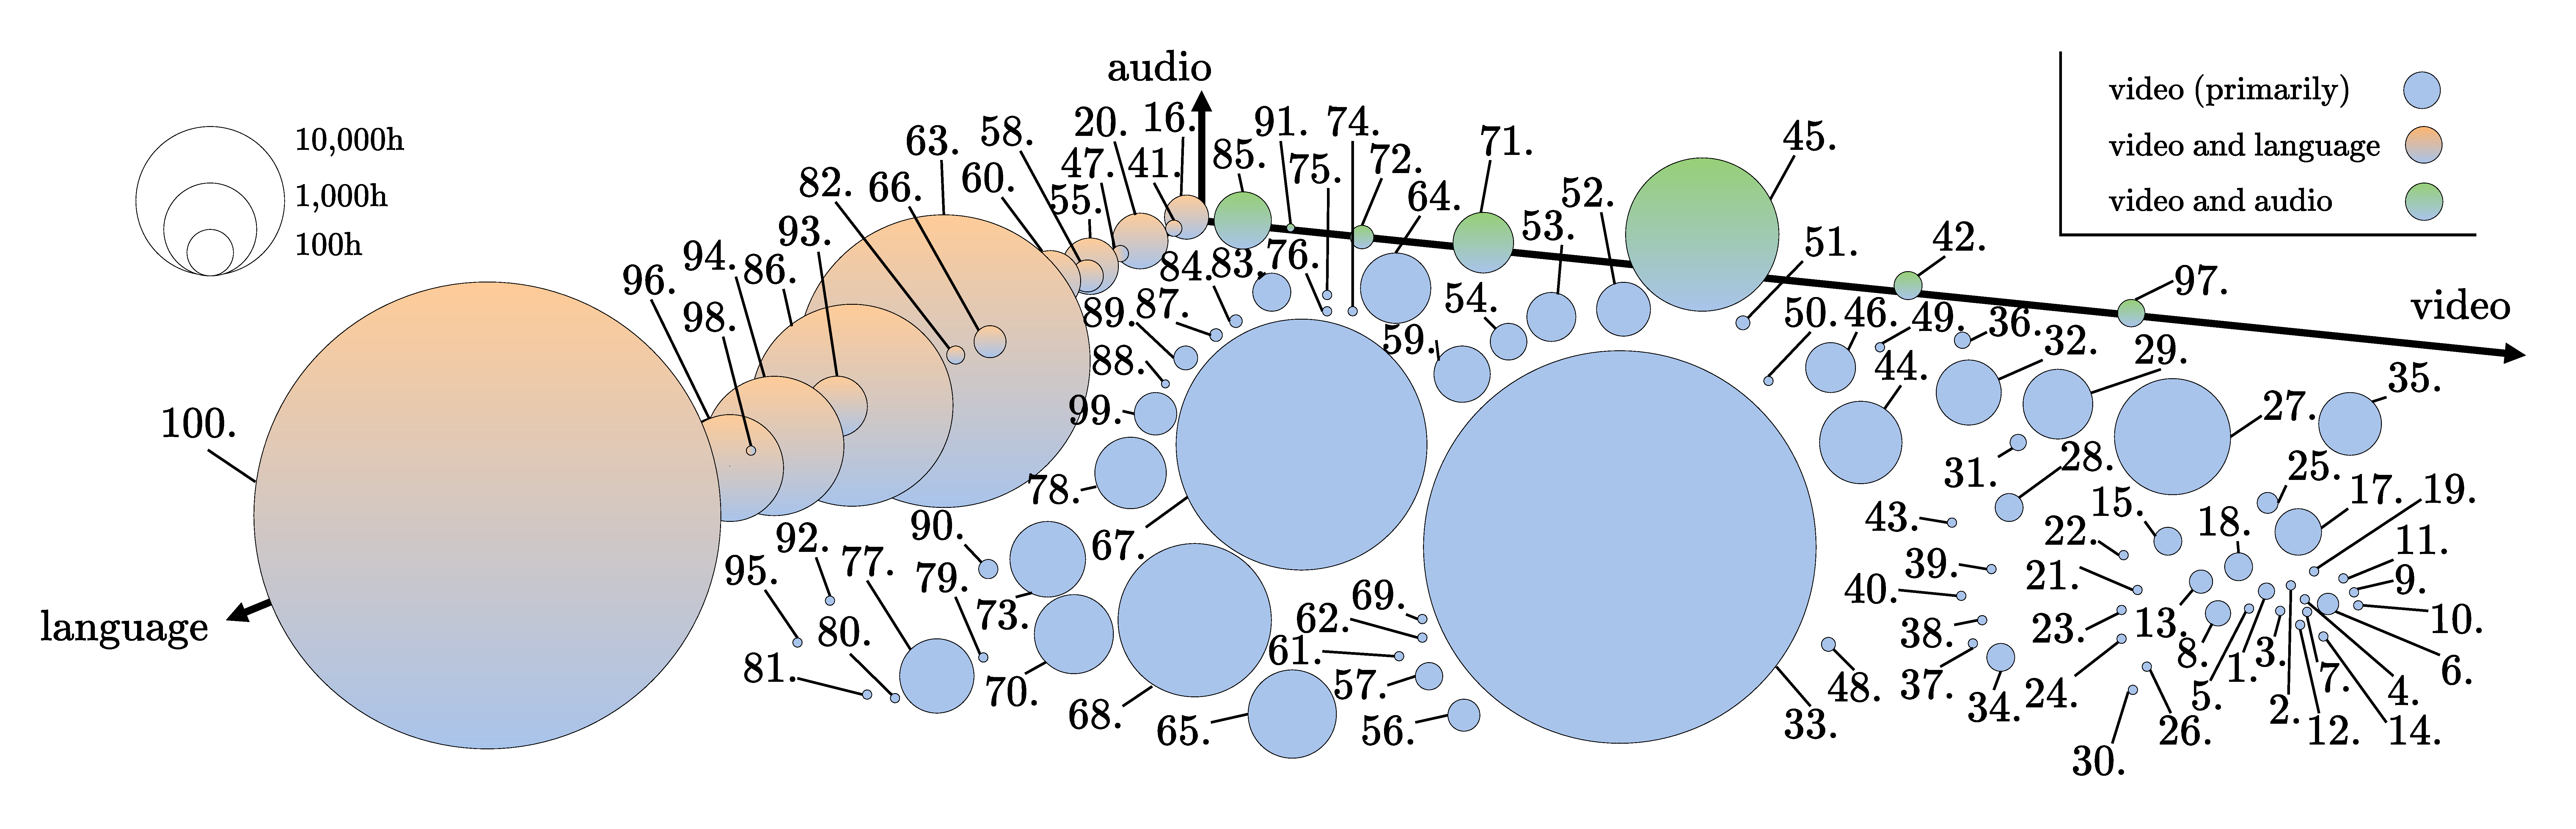
\includegraphics[width=\linewidth]{figs/datasets.pdf}
    \resizebox{\linewidth}{!}{
    \begin{tabular}{llll}
      1. KTH~\citep{schuldt2004recognizing} &  
      2. Weizmann~\citep{gorelick2007actions} &  
      3. Coffee \& Cigarettes~\citep{laptev2007retrieving} & 
      4. CASIA Action~\citep{wang2007human} \\ 
      5. UCF Sports~\citep{rodriguez2008action} & 
      6. Hollywood~\citep{laptev2008learning} & 
      7. UT-Interaction~\citep{ryoo2009spatio} & 
      8. CMU-MMAC~\citep{deguide2008guide} \\
      9. UCF-11~\citep{liu2009recognizing} & 
      10. Hollywood2~\citep{marszalek2009actions} & 
      11. TV-HI~\citep{patron2010high} &
      12. Humaneva~\citet{sigal2010humaneva} \\
      13. UCF-50~\citep{reddy2013recognizing} & 
      14. Olympic Sports~\citep{niebles2010modeling} &
      15. HMDB-51~\citep{kuehne2011hmdb} &
      16. MSVD~\citep{chen2011collecting} \\
      17. CCV~\citep{jiang2011consumer} & 
      18. UCF-101~\citep{soomro2012ucf101} &
      19. CAD-60~\citep{sung2012unstructured} &
      20. MPII~\citep{rohrbach2012database} \\ 
      21. ADL~\citep{pirsiavash2012detecting} &
      22. 50 Salads~\citep{stein2013combining} &
      23. AVENUE~\citep{lu2013abnormal} &
      24. J-HMDB~\citep{jhuang2013towards} \\
      25. CAD-120~\citep{koppula2013learning} &
      26. Penn Action~\citep{zhang2013actemes} &
      27. Sports-1M~\citep{karpathy2014large} & 
      28. EGTEA Gaze+~\citep{li2015delving} \\
      29. ActivityNet-100~\citep{caba2015activitynet} &
      30. Watch-n-Patch~\citep{wu2015watch} &
      31. NTU-RGB-60~\citep{shahroudy2016ntu} &
      32. ActivityNet-200~\citep{caba2015activitynet} \\
      33. YouTube-8M~\citep{abu2016youtube} &
      34. Charades~\citep{sigurdsson2016hollywood} &
      35. ShakeFive2~\citep{van2016spatio} &
      36. DALY~\citep{weinzaepfel2016towards} \\
      37. OA~\citep{li2016recognition} &
      38. CONVERSE~\citep{edwards2016pose} &
      39. TV-servies~\citep{de2016online} & 
      40. Volleyball~\citep{ibrahim2016hierarchical} \\
      41. MSR-VTT~\citep{xu2016msr} &
      42. Greatest Hits~\citep{owens2016visually} &
      43. Okutama Action~\citep{barekatain2017okutama} &
      44. K-400~\citep{kay2017kinetics} \\
      45. AudioSet~\citep{gemmeke2017audio} &
      46. Smthng-Smthng (v1/v2)~\citep{goyal2017something} &
      47. TGIF~\citep{jang2017tgif} &
      48. CMU Panoptic~\citep{joo2017panoptic} \\
      49. MultiTHUMOS~\citep{yeung2018every} &  
      50. RESOUND~\citep{li2018resound} &
      51. EK-55~\citep{damen2018scaling} &
      52. K-600~\citep{carreira2018short} \\
      53. VLOG~\citep{fouhey2018lifestyle} &
      54. AVA~\citep{gu2018ava} &
      55. TVQA~\citep{lei2018tvqa} &
      56. UCF-Crime~\citep{sultani2018real} \\
      57. Charades-Ego~\citep{sigurdsson2018charades} &
      58. YouCook2~\citep{zhou2018towards} &
      59. K-700~\citep{carreira2019short} &
      60. COIN~\citep{tang2019coin} \\
      61. AIST~\citep{tsuchida2019aist} &
      62. Drive\&act~\citep{martin2019drive} &
      63. HowTo100m~\citep{miech2019howto100m}&
      64. Moments in Time~\citep{monfort2019moments} \\
      65. HACS~\citep{zhao2019hacs} &
      66. VATEX~\citep{wang2019vatex} &
      67. IG65M~\citep{ghadiyaram2019large} &
      68. Toyota Smarthome~\citep{dai2022toyota} \\
      69. OOPS~\citep{epstein2020oops} &
      70. AViD~\citep{piergiovanni2020avid} &
      71. VGGSound~\citep{chen2020vggsound} &
      72. LLP~\citep{tian2020unified} \\
      73. HVU~\citep{diba2020large} &
      74. DMP~\citet{ortega2020dmd} &
      75. Action Genome~\citep{ji2020action} &
      76. Countix~\citep{dwibedi2020counting} \\
      77. K-700 (2020)~\citep{smaira2020short} &
      78. FineGym~\citep{shao2020finegym} & 
      79. RareAct~\citep{miech2020rareact} &
      80. Immersive Light Field~\citet{broxton2020immersive} \\
      81. HAA500 \citep{chung2021haa500} &
      82. IKEA ASM~\citep{ben2021ikea} &
      83. MultiSports~\citep{li2021multisports} &
      84. MOMA~\citep{luo2021moma} \\
      85. Spoken Moments~\citep{monfort2021spoken} &
      86. WebVid-2M~\citep{bain2021frozen} &
      87. Home action genome~\citep{rai2021home} & 
      88. DanceTrack~\citep{sun2022dancetrack} \\
      89. EK-101~\citep{damen2022rescaling} &
      90. FineAction~\citep{liu2022fineaction} &
      91. AVSBench~\citep{zhou2022audio} &
      92. Neural 3D Video~\citet{li2022neural} \\
      93. Assembly101~\citep{sener2022assembly101} &
      94. Ego4D \citep{grauman2022ego4d} &
      95. SportsMOT~\citep{cui2023sportsmot} &
      96. Ego-Exo-4D \citep{grauman2024ego} \\ 
      97. EPIC-Sounds \citep{huh2023epic} &
      98. MVBench \citep{li2024mvbench} &
      99. OVR \citep{dwibedi2024ovr} \\
      100. Vidchapters-7M \citep{yang2024vidchapters}
    \end{tabular}
    }
    \caption{\textbf{Comparisons of total dataset duration and primary modality}. Circle sizes correspond to the (approximate) summed duration of all videos in the datasets. Recent datasets (i.e., $>80$) have longer total running times and include additional modalities such as language or audio.}
    \label{fig:dataset_blobs}
\end{figure*}

\subsection{General datasets}
\label{sec:datasets::general}
The past two decades have seen datasets with increased number of available videos that in turn lead to new and more robust baselines. We present widely-adopted benchmarks chronologically in \Cref{tab:action_recognition_datasets}. Initial efforts \citep{schuldt2004recognizing,gorelick2007actions} have primarily focused on categorizing atomic, low-motion-magnitude actions such as \emph{walking} and \emph{hand waving}. Subsequent datasets predominantly comprised videos from either TV shows/movies \citep{laptev2007retrieving,laptev2008learning,marszalek2009actions,patron2010high,kuehne2011hmdb} or sports \citep{rodriguez2008action,liu2009recognizing,reddy2013recognizing,niebles2010modeling}. A step towards establishing large-scale datasets for the video domain was made with the introduction of Sports-1M \citep{karpathy2014large}, YouTube-8M \citep{abu2016youtube}, and Kinetics \citep{carreira2017quo} that include web-sourced videos over diverse sets of actions. Evident from their sizes shown in \Cref{fig:dataset_blobs}, these datasets paved the way as general benchmarks for models that can be adapted for action-type-specific smaller datasets such as UCF-101 \citep{soomro2012ucf101} and ActivityNet \citep{caba2015activitynet}. Despite their size and use for multiple downstream tasks, there is still room to address specific action understanding tasks or modalities supplementary to vision.  Domains such as 
egocentric vision, human-object interactions, and hierarchical action understanding have also gained popularity prompting the creation of domain-specific datasets. EGTEA Gaze+ \citep{li2015delving}, EPIC KITCHENS \citep{damen2022rescaling}, and later EGO4D \citep{grauman2022ego4d} have been the main datasets and benchmarks for egocentric vision. Similarly, Something-Something \citep{goyal2017something} and Charades \citep{sigurdsson2016hollywood} have been used as benchmarks for object-based actions with a greater focus on temporal information. Datasets such as Diving-48 \citep{li2018resound} and FineGym \citep{shao2020finegym} incorporate semantic hierarchies in their annotations. More recent datasets have focused on tasks related to action recognition including instruction learning \citep{alayrac2016unsupervised,bansal2022my,ben2021ikea,ohkawa2023assemblyhands,sener2022assembly101,tang2019coin}, action phase alignment \citep{sermanet2017unsupervised}, repeating action counting \citep{dwibedi2020counting,dwibedi2024ovr,hu2022transrac,runia2018real,zhang2020context}, action completion prediction \citep{epstein2020oops}, driver behavior recognition \citep{martin2019drive,ortega2020dmd}, anomaly detection \citep{acsintoae2022ubnormal,liu2018future,lu2013abnormal,sultani2018real,wu2020not}, hand-object interactions \citep{chao2021dexycb,garcia2018first,hampali2020honnotate,kwon2021h2o,moon2020interhand2,mueller2017real}, and object state changes in actions \citep{souvcek2022look}. 



\subsection{Domain- and modality-specific datasets}
\label{sec:datasets::specific}

Apart from general-purpose datasets, several benchmarks have been designed to evaluate model capabilities of specific aspects of action understanding. We overview three groups of domains and benchmarks based on the holistic understanding of scenes from multiple viewpoints with supplementary modalities such as language and audio.

% Multi-view and multi-camera set-ups
\noindent
\textbf{Multi-view}. Initial efforts to compile multi-view videos included a small number of subjects \citep{sigal2010humaneva} or synthetic data \citep{ionescu2013human3}. High-quality multi-view videos are highly dependent on the hardware and setup \citep{wang2023learning}. CMU panoptic \citep{joo2017panoptic} captured group interactions within a dome with 480 VGA cameras. Interactions included social settings, games, dancing, and musical performances. ZJU-Mocap \citep{peng2021neural} comprised dynamic videos of human motions from 20 cameras. The Immersive Light Field dataset \citep{broxton2020immersive} contains light field videos with 6 degrees of freedom with a camera rig consisting of 46 action cameras. Multi-view datasets are collected for a variety of target tasks, including 3D video synthesis of human actions and interactions in indoor \citep{li2022neural} and outdoor \citep{lin2021deep,yoon2020novel} settings, dance sequence reconstruction \citep{tsuchida2019aist}, and the dynamic synthesis of indoor spaces in which actions take place \citep{tschernezki2024epic}.

% Language-related datasets
\noindent
\textbf{Video-language}. In recent years, language has been integrated into vision methods as a natural extension to represent high-level semantics. Commonly, learning to map textual concepts and visual representations in a shared embedding space has been a widely adopted strategy by many video tasks \citep{amrani2021noise,gabeur2020multi,liu2019use,miech2020end}. Initial video-language datasets \citep{chen2011collecting,xu2016msr} were based on short video snippets and short textual descriptions of actions with more recent efforts also providing multilingual descriptions \citep{wang2019vatex}. Video question-answering is a popular language-based task explored in a large number of works \citep{jang2017tgif,lei2018tvqa,li2024mvbench,oncescu2021queryd,xiao2021next}. The order of instructions has been of great interest in longer videos since the introduction of HowTo100M \citep{miech2019howto100m} and YouCook2 \citep{zhou2018towards}. Benchmarks have also been proposed for other long-form tasks such as moment retrieval \citep{song2024moviechat,yang2024vidchapters}, and long-term reasoning \citep{mangalam2023egoschema}.

% Video and audio
\noindent
\textbf{Audio and vision}. Human perception has often relied on both vision and audio for understanding actions, especially in conditions where appearance may lead to ambiguous predictions. Audioset \citep{gemmeke2017audio} is the largest audio-visual action dataset containing 2.1M clips across a long-tail distribution of 527 classes. VGG-Sound \citep{chen2020vggsound} is another common benchmark with a uniform distribution of 200K videos over 300 classes. Datasets have also been collected for specific tasks such as audio-visual semantic segmentation \citep{zhou2022audio}, audio-visual video parsing \citep{tian2020unified}, materials sound and action classification \citep{huh2023epic,owens2016visually}, and video captioning \citep{monfort2021spoken}.

% link to next section
The introduction of both general and task-specific datasets has enabled better exploration of video tasks through the availability of common data and standardized evaluation protocols. The main lines of research for these tasks alongside their challenges are overviewed next.